\chapter{Foundations}\label{foundations}
Most of the groundwork of the methods we will be using was invented in the second half of the 20th century. They include reinforcement learning---a general framework defining the aim of the playing algorithm, Q-learning---a simple algorithm to learn to play a game, and basics of neural networks---the statistical model that was used to overcome Q-learning's limitations.
This foundation work, joined with the recent (after $2010$) advances in the methods of training and architectures of neural networks allowed to vastly improve the former results.

This chapter discusses these methods, as well as describes the Atari machine, as the games we are interested in playing are created for this platform.

\section{Reinforcement learning}
To create an algorithm learning to play a game or solve any other problem, we first have to formally define what the problem is. We will model Atari games within the framework called reinforcement learning. The main property distinguising reinforcement learning problems from supervised learning (prediction) and unsupervised learning (clustering) is presence of two separate entities: the \emph{environment} and the \emph{agent}.

The environment is the physics or the rules of the game. It presents state, which can be any description of the game, to the agent, scores its action and provides him with the following state.
The agent is the algorithm we prepare. It receives a state it is in from the environment, decides which action to choose there and receives the appropriate reward. Every move happens in a discrete moments of time.

The aim of the creator of the reinforcement learning algorithm is to invent a way to map the game state for each time $t$: $s_t$ to the action $a_t$ (possibly storing some inner state), so that the sum:
\begin{equation} \label{discounted-reward}
\sum_{k=0}^{\infty} \gamma^k r_{t + k}
\end{equation}
is maximized. $r_T$ is the reward received after doing action $a_T$ in state $s_T$ The exponential averaging is called a \emph{discounted} sum, and $0 < \gamma \le 1$ is called a \emph{discount factor} corresponds to the level of comfort we have with receiving the awards not now, but in the future. This resembles the way people evaluate their gains---if one is promissed a constant amount of money, he'd prefer to receive it rather earlier than later. We assume that every game eventually will find itself in a \emph{terminal} state, which always transistions to a terminal state and gives reward $0$. One such progression from the start of the game to reaching a terminal state is called an \emph{episode}.

Both agent and environment are not bound to make their decisions deterministically---in fact, it may be favorable for the agent to play randomly to some extent. In the stochastic case, the aim of the agent is to maximize the discounted sum of expected value of the rewards.

\begin{figure}[!h]
  \center
  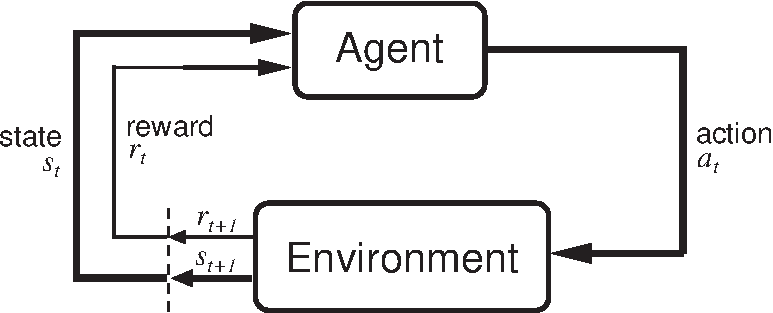
\includegraphics[scale=0.8]{images/Agent-Env-crop.pdf}
  \caption{The interaction between the agent and the environment, from \cite{reinforcement-book}.}
\end{figure}

The reinforcement learning, as defined above is a very general framework which can describe a broad range of problems. To make it easier to model it using statistical tools, we assume all the problems we consider are of the form of Markov Decision Process.

Markov Decision Process (MDP) is a reinforcement learning problem where a distribution of the following states $s_{t+1}$ and the rewards $r_t$ depends only on the previous state $s_t$ and the action $a_t$ (we assume reward $r_t$ is rewarded after choosing action $a_t$):
\begin{equation} \label{mdp}
  p(s_{t+1}, r_t|s_t, a_t, s_{t-1}, a_{t-1}, \ldots, s_0, a_0) = p(s_{t+1}, r_t|s_t, a_t)
\end{equation}

This simplifying assumtion can be summarized as "agent has all the information he needs for making actions encoded in the state". One should note that the representation of the state and not the inner mechanics of environment, is crucial here---imagine a chess-playing player, which sees only bottom half of the board. Even though the game is completely deterministic (assuming deterministic strategy of agent and environment, choosing oppontents' moves), agent cannot reliably predict what will be the next state, as there may be pieces on the other part of the board he cannot see yet.

In the case of Atari games played based on the RAM state, the MDP assumptions are satisfied. The code of the game (saved on ROM), together with a random seed for the game define a deterministic function transforming the RAM (the game state) and awarding rewards.

It is worth noting that the algorithms based on markovian assumption (TD-learning, Q-learning, Markov Chain Monte Carlo) are often used dispite the violation of assumption by the environment. The intuition behind that when the state contains enough information for agent to reasonably approximate the next state and reward distribution, it doesn't matter the approximation will not be accurate. One example of this fact is when we train agents to play Atari games based on the screen state \cite{nips-dqn}---the player moves influence the inner state (RAM) of the machine, but the changes may not be immediately apparent on the screen. Still, the game screen gives a lot of information about the game state needed to make an action, thus 
agent can fairly skillfully learn to make good decisions.

\section{Q-learning}
Let's call the function (distribution) mapping the current state $s$ to the action $a$ choosen by the agent \emph{a strategy} (or \emph{policy}) $\pi$.

An algorithm able to choose a strategy in an MDP we will discuss is called Q-learning \cite{qlearning, qlearning-old}. It is based on the notion of Q-value: a function mapping the state-action pair $(s, a)$, for a fixed strategy $\pi$ to the expected discounted reward after being in the state $s$, making an action $a$ and following the strategy $\pi$ until the end of the episode.
\begin{equation}\label{q-value}
  Q^\pi(s_t, a_t) = \underset{r\sim p(r_t | s_t, a_t)}{\mathbb{E}} r + \sum_{k=t+1}^\infty \gamma^{k-t}\underset{r\sim p(r_k|s_{k-1}, a_{k-1}), a_k\sim \pi(s_k)}{\mathbb{E}} r
\end{equation}
where $s_k$ is a random variable describing distribution of the state in time $k$, dependent of the previous state and action, as in equation \eqref{mdp}. From here on, though, we will assume that choice of the next states and rewards by the envirnoment as well as of actions by the agent are done deterministically---it will simplify the notation and all the statements will hold for the stochastic case when wrapped with the expectation signs.

The Q-learning algorithm makes use of the following property:
The strategy $\pi$ is optimal (maximizes the expected discounted reward) if and only if
\begin{equation}\label{qlearning-property}
  Q^\pi(s_t, a_t) = r_t + \gamma \max_a Q(s_{t+1}, a)
\end{equation}
for all state-action pairs.
\todo[noinline]{Maybe prove that fact: left -- for optimal strategy we can do greedy actions, right -- assume strategy is not optimal but property satisfied, then there's a better strategy that does different action somewhere, but this action leads to lower Q}

Q-learning is a representative of a general domain of algorithms called Generalized Policy Iteration (see ch. 4.6. in \cite{reinforcement-book}). Their approach is to take turns between updating the estimation of the value of the states (in our case Q-values) and updating the strategy to take into account new state value estimation.
 
In case of Q-learning, the chosen strategy is a greedy one, i.e. it always chooses the action maximizing the immediate reward plus discounted value of the following state:
\begin{equation}
  \pi(s_t) = \argmax_a \big(r(s_t, a) + \max_{a^*} Q^\pi(s_{t+1}, a^*)\big)
\end{equation}
where $r(s, a)$ is the immediate reward after making action $a$ in state $s$ and $s_{t+1}$ is a (convenient notation for a) next state after making action $a$ in state $s_t$.

The update to the Q-values is being made to force more state-action pairs to satisfy property \eqref{qlearning-property}:
\begin{equation}
  Q_{new}(s_t, a) := \alpha Q_{old}(s_t, a) + (1 - \alpha)\big(r(s_t, a) + \max_{a^*} Q_{old}(s_{t+1}, a^*)\big)
\end{equation}
$\alpha$ (also called step-size) is a parameter of the algorithm deciding how fast should it move the q-value estimations toward the ones locally satisfying \eqref{qlearning-property}. Bigger values lead to faster training, but the convergence proof for constant step-size requires sufficiently small $\alpha$ \cite[section~3.]{qlearning-old}. It was also shown in \cite{qlearning-convergence}, that the Q-learning algorithm converges when the variable step-size satisfies:
\begin{equation}
  \sum_i \alpha_i = \infty, \;\;\;\; \sum_i \alpha_i^2 < \infty
\end{equation}

Assuming we store all the state transitions as $next\_state[s, a]$ and the rewards as $reward[s, a]$\footnote{in the non-deterministic case these can be approximated by, respectively, observed distribution of the next states and the sample average of rewards in each state-action pair}, the Q-learning algorithm can be written as:

\begin{algorithm} \label{qlearning-pseudo}
  \For{all state-action pairs$ (s, a)$}{
    $Q[s, a] = 0$ \tcp{ initialize Q-values of all state-action pairs}
  }
  \For{all states $s$}{
    $P[s] = random\_action()$ \tcp{ initialize strategy}
  }
  \While{not converged}{
    \For{all states $s$}{
      $P[s] = \argmax_a (R[s, a] + \gamma \max_b(Q[next\_state[s, a], b]))$
    }
    \For{all state-action pairs$ (s, a)$}{
      $Q[s, a] = \alpha(R[s, a] + \gamma \max_b Q[next\_state[s, a], b]) + (1 - \alpha)Q[s, a]$
    }
  }
  \caption{Pseudocode of Q-learning.}
\end{algorithm}
\section{Deep Learning}
\todo{Tell that this chapter defines deep learning, which is a set of machine learning methods invented recently, owning state-of-the-arts methods in many domains}
\todo{Shortly cite some results}
\subsection{Neural networks}
\todo{Define neural network}
\todo{Cite some early works}

\subsection{Deep Learning revolution}
\todo{Tell that these methods were not considered state-of-the-art models until recently}
\todo{Tell that there came much faster GPUs, which allowed to have deeper networks evaluated quickly}
\todo{Tell that there were invented algorithms that better move in the multidimensional space of parameters, faster converging to a better local minimum}
\todo{Tell that it was not expected and cite Krizhevsky paper}

\todo{Tell about libraries: Torch, Theano, Tensorflow, the latter two allow for automatic differentiation}
\todo{Tell about libraries built on top of these: Keras, blocks, TFLearn}

\section{Atari 2600}
\todo{Tell about the "architecture" of the Atari machine}
\todo{Tell about the different games}
\todo{Tell about creation of ALE}
\todo{Tell about creation of OpenAI}
